%!TEX program = xelatex
% 完整编译: xelatex -> bibtex -> xelatex -> xelatex
\documentclass[lang=cn,12pt,a4paper,cite=authoryear]{elegantpaper}

\title{粒子群优化算法浅析及其在经济管理领域的应用}
\author{李子岳 \\ 经71 \\ 2017012781 \and 肖昌荣 \\ 经71 \\ 2017012527}
%\institute{清华大学经济管理学院}

%\version{0.09}
\date{\zhtoday}


% 本文档命令
\usepackage{array}
\newcommand{\ccr}[1]{\makecell{{\color{#1}\rule{1cm}{1cm}}}}
\usepackage{booktabs}
\usepackage{float}
\linespread{1.5}
\usepackage[noend]{algpseudocode}
%\usepackage{algorithmicx, algorithm}
\usepackage[ruled]{algorithm2e}

\begin{document}

\maketitle

\begin{abstract}
粒子群算法(PSO)是一种优化问题得到最优解的元启发算法,受到自然界中鸟群活动的启发,有非常简洁的结构,而且在实际中取得了非常广泛的应用。本文介绍了粒子群算法的实现原理,并通过代码模拟的方式解释了PSO算法的操作流程,以运营管理中常见的情景为例,得到了优化的结果。文章介绍了PSO算法在经济管理领域的应用,并分析了该算法的现状以及未来可能的发展与研究方向。
\keywords{粒子群优化算法,运营管理}
\end{abstract}

\section{算法简介}

粒子群优化(Particle Swarm Optimization, PSO),又称微粒群算法,是由 \cite{kennedy1995particle}于1995年开发的一种演化计算技术。它是一种元启发法,对于要优化的问题只需要做出很少或根本不需要假设、不使用要优化问题的梯度,这意味着PSO不需要像经典的优化方法(例如梯度下降和拟牛顿法)所要求的那样使优化问题可微分。所以算法的适用范围更广,可以搜索很大范围的候选解决方案。

粒子群优化算法来源于对鸟群行为社会模型的模拟。其中“群(swarm)”来源于微粒群, “粒子(particle)”则是一个折衷的选择,因为既需要将群体中的成员描述为没有质量、没有体积的,同时也需要描述它的速度和加速状态。算法主要源于两种思想方法,首先是它与人工生命的联系,例如鸟群、鱼群、蚁群等群体理论(Swarming Theory)。其次,它也与进化计算有关,特别是遗传算法和进化编程\citep{kennedy1995particle}。

PSO是一个极为简单且十分有效地适用于许多优化问题中的优化算法,它在多维空间函数寻优、动态目标寻优等方面有着收敛速度快、解质量高、鲁棒性好等优点,特别适合于工程应用\citep{huanglei}。但是PSO作为一种元启发法不能保证找到最佳解决方案,且存在与算法收敛性相关的问题。这些缺陷并不妨碍粒子群优化算法成为最为经典的智能算法之一,许多学者同样受到自然界启发,开发了诸多类似的智能算法,且PSO从提出至今不断有学者对其进行完善,提高其在实际应用中的效果。


\section{算法原理与实现}

\subsection{算法原理}

粒子群优化算法受到自然界中鸟群的启发,它考虑的情景是,在一个区域内有大大小小不同的食物源,鸟群的任务是找到最大的食物源。鸟群在整个搜寻的过程中,通过相互传递各自位置的信息,让其他鸟知道食物源的位置,最终整个鸟群都能聚集在最大食物源周围,即找到了全局最优解,问题收敛。


\begin{figure}[H]
	\centering
	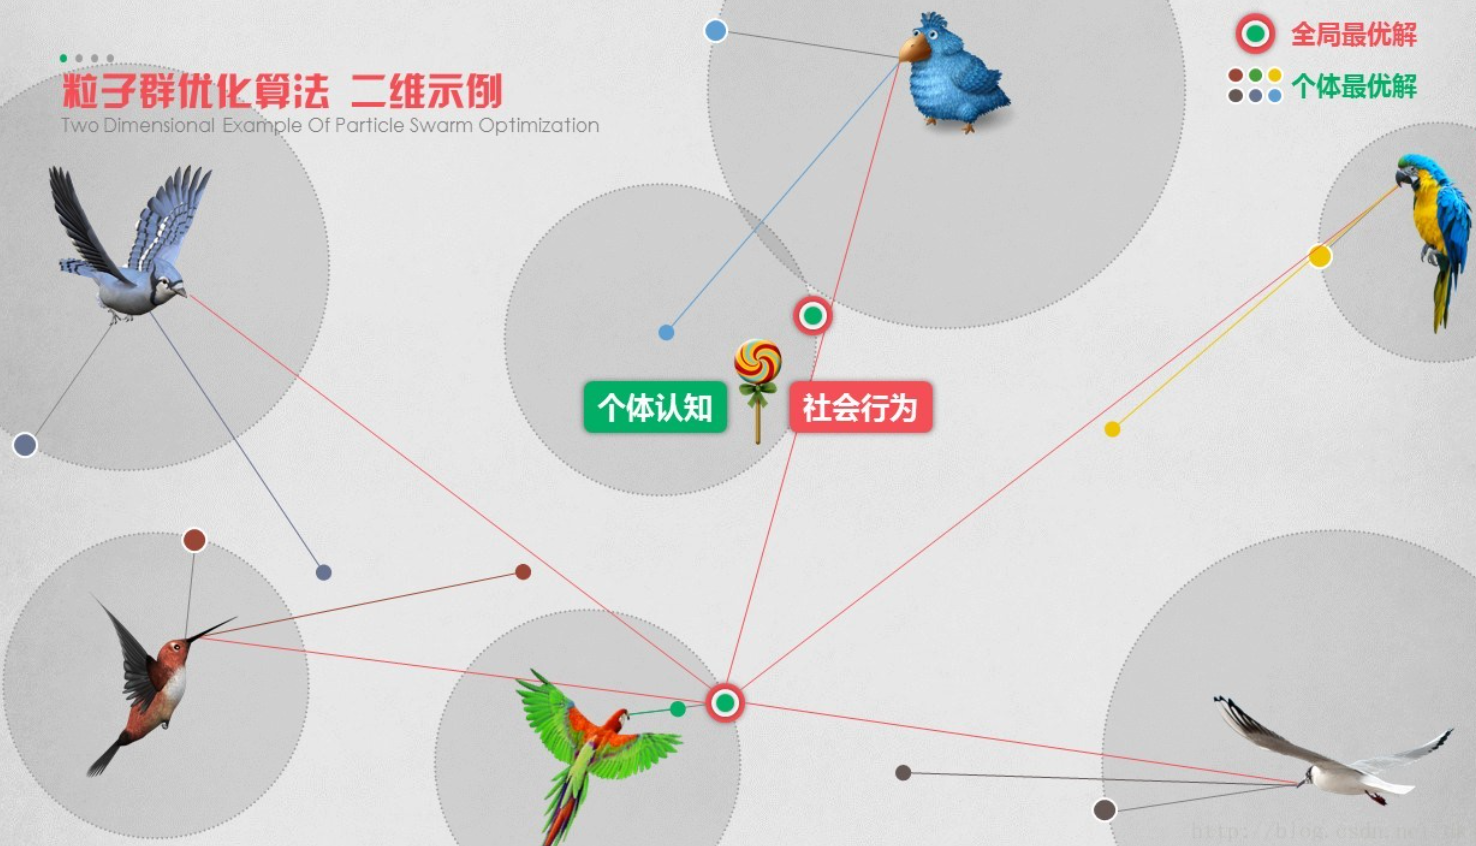
\includegraphics[width=0.6\textwidth]{image/psointro.png}
	\caption{PSO算法示例}
	\label{psointro}
\end{figure}





为了找到食物源,一群鸟在森林里漫无目的的飞着,假设他们能感知到自己距离食物的距离。A是这群鸟中的一只,它从其他同伴的口中得知,当前鸟B距离食物最近,所以它考虑着往鸟B的方向飞。但是,鸟A突然想到,虽然现在鸟B距离食物最近,但自己曾经飞过的位置Z是已经飞过的路途中距离食物最近的点。现实情况中,食物源可能与Z点距离更近,也可能与鸟B与距离更近。因此,一般性原则是,鸟A选择朝着鸟B和朝着位置Z的方向的矢量和的方向飞行,这就是下文算法中提到的速度更新公式。
$$v_{id} = v_{id} + c_1 * rand() * (p_{id} - x_{id}) + c_2 * Rand() * (p_{gd} - x_{id})$$

我们把上式中的$c_1$称为社会学习因子,$c_2$称为个体学习因子。使用上述速度更新公式,鸟A就知道自己应该朝哪个方向飞行,所以就得到下面的位置更新公式。
$$x_{id} = x_{id} + v_{id}$$


\begin{figure}[H]
	\centering
	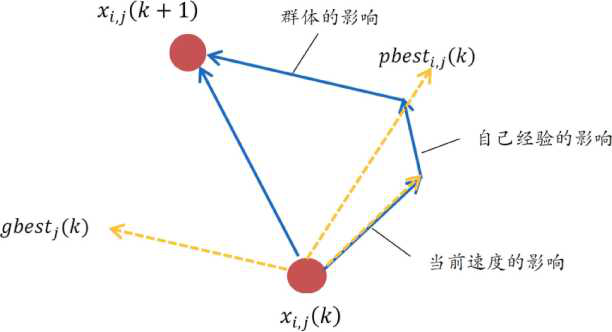
\includegraphics[width=0.6\textwidth]{image/pso_algorithm.png}
	\caption{PSO更新过程}
	\label{psointro}
\end{figure}



将上述描述抽象为算法模型,\cite{shi2001particle}在文章中给出的算法如下:

~\\

\begin{algorithm}[H]
	\caption{Particle Swarm Optimization}
	{\textbf{Initialize} a population of particles with random positions $x_{id}$ and velocities $v_{id}$ on a $d$ dimensions problem space}\\
	\While{the criterion is not met}{
		\ForEach{particle}{
			evaluate the desired optimization fitness function\\
			compare particle's fitness evaluation with particle's $pbest$\\
			\If{current value is better than $pbest$}{
				$pbest \text{ value} = \text{current value}$\\
				$pbest \text{ location} = \text{current location}$
			}
			compare particle's fitness evaluation with population's overall $gbest$\\
			\If{current value is better than $gbest$}{
				$gbest \text{ value} = \text{current value}$\\
				$gbest \text{ location} = \text{current location}$\\
				$gbest \text{ index} = \text{current index}$
			}
			update the velocity and position of the particle\\
			$v_{id} = v_{id} + c_1 * rand() * (p_{id} - x_{id}) + c_2 * Rand() * (p_{gd} - x_{id})$\\
			$x_{id} = x_{id} + v_{id}$
		}
	}
	
\end{algorithm}

%~\\

简而言之,算法首先规定变量的取值范围并给出目标函数,初始化粒子群中各个粒子的初始位置、初始速度等参数,接着依据目标函数计算每个粒子的适应度,根据适应度更新粒子自身最佳位置$pbest$和群体最佳位置$gbest$,如此循环直至满足全局最优条件或到达迭代次数上限。简化的直观流程如下图(\ref{fig1})所示:

\begin{figure}[H]
	\centering
	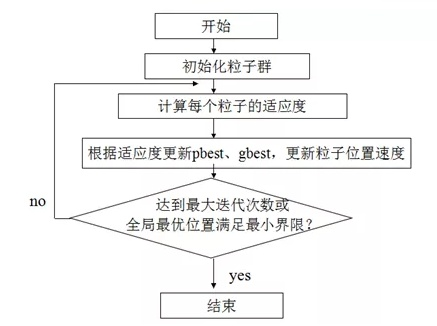
\includegraphics[width=0.6\textwidth]{image/algorithm.jpg}
	\caption{PSO算法流程图}
	\label{fig1}
\end{figure}

可以看出,随着计算的推移,通过探索和利用搜索空间中已知的有利位置,粒子围绕一个或多个最优点聚集或聚合。该算法设计玄妙之处在于它保留了最优全局位置和粒子已知的最优位置两个信息。后续的实验发现,保留这两个信息对于较快收敛速度以及避免过早陷入局部最优解都具有较好的效果。这也奠定了后续粒子群算法改进方向的基础。

\subsection{算法实例}

在这一部分,我们使用Python实现粒子群优化算法在简单问题中的应用,评估算法的表现。

\subsubsection{例一}

首先我们将所要优化的目标函数设为一个简单的二元函数:
$$\min y = \frac{1}{100}(x_1^2 + x_2^2)$$

其中$x_1$和$x_2$的取值范围为
$$x_1 \in [-300, 300], \quad x_2 \in [-300, 300]$$

将个体学习因子$c1$和社会学习因子$c2$都定为0.5,设置粒子群大小为50、迭代上限为200次,利用PSO算法求解该优化问题,得到最优结果为:
$$x_1^*=-1.1057,\ x_2^*=-0.3589,\ y^*= 0.0135$$

十分接近理论最优值0。图(\ref{fig2})为目标函数值随迭代次数的变化,我们发现算法在大约75次迭代就能达到最优,所以无论从运行时间还是优化精度来说,粒子群优化算法的都是较为高效的。

\begin{figure}[H]
	\centering
	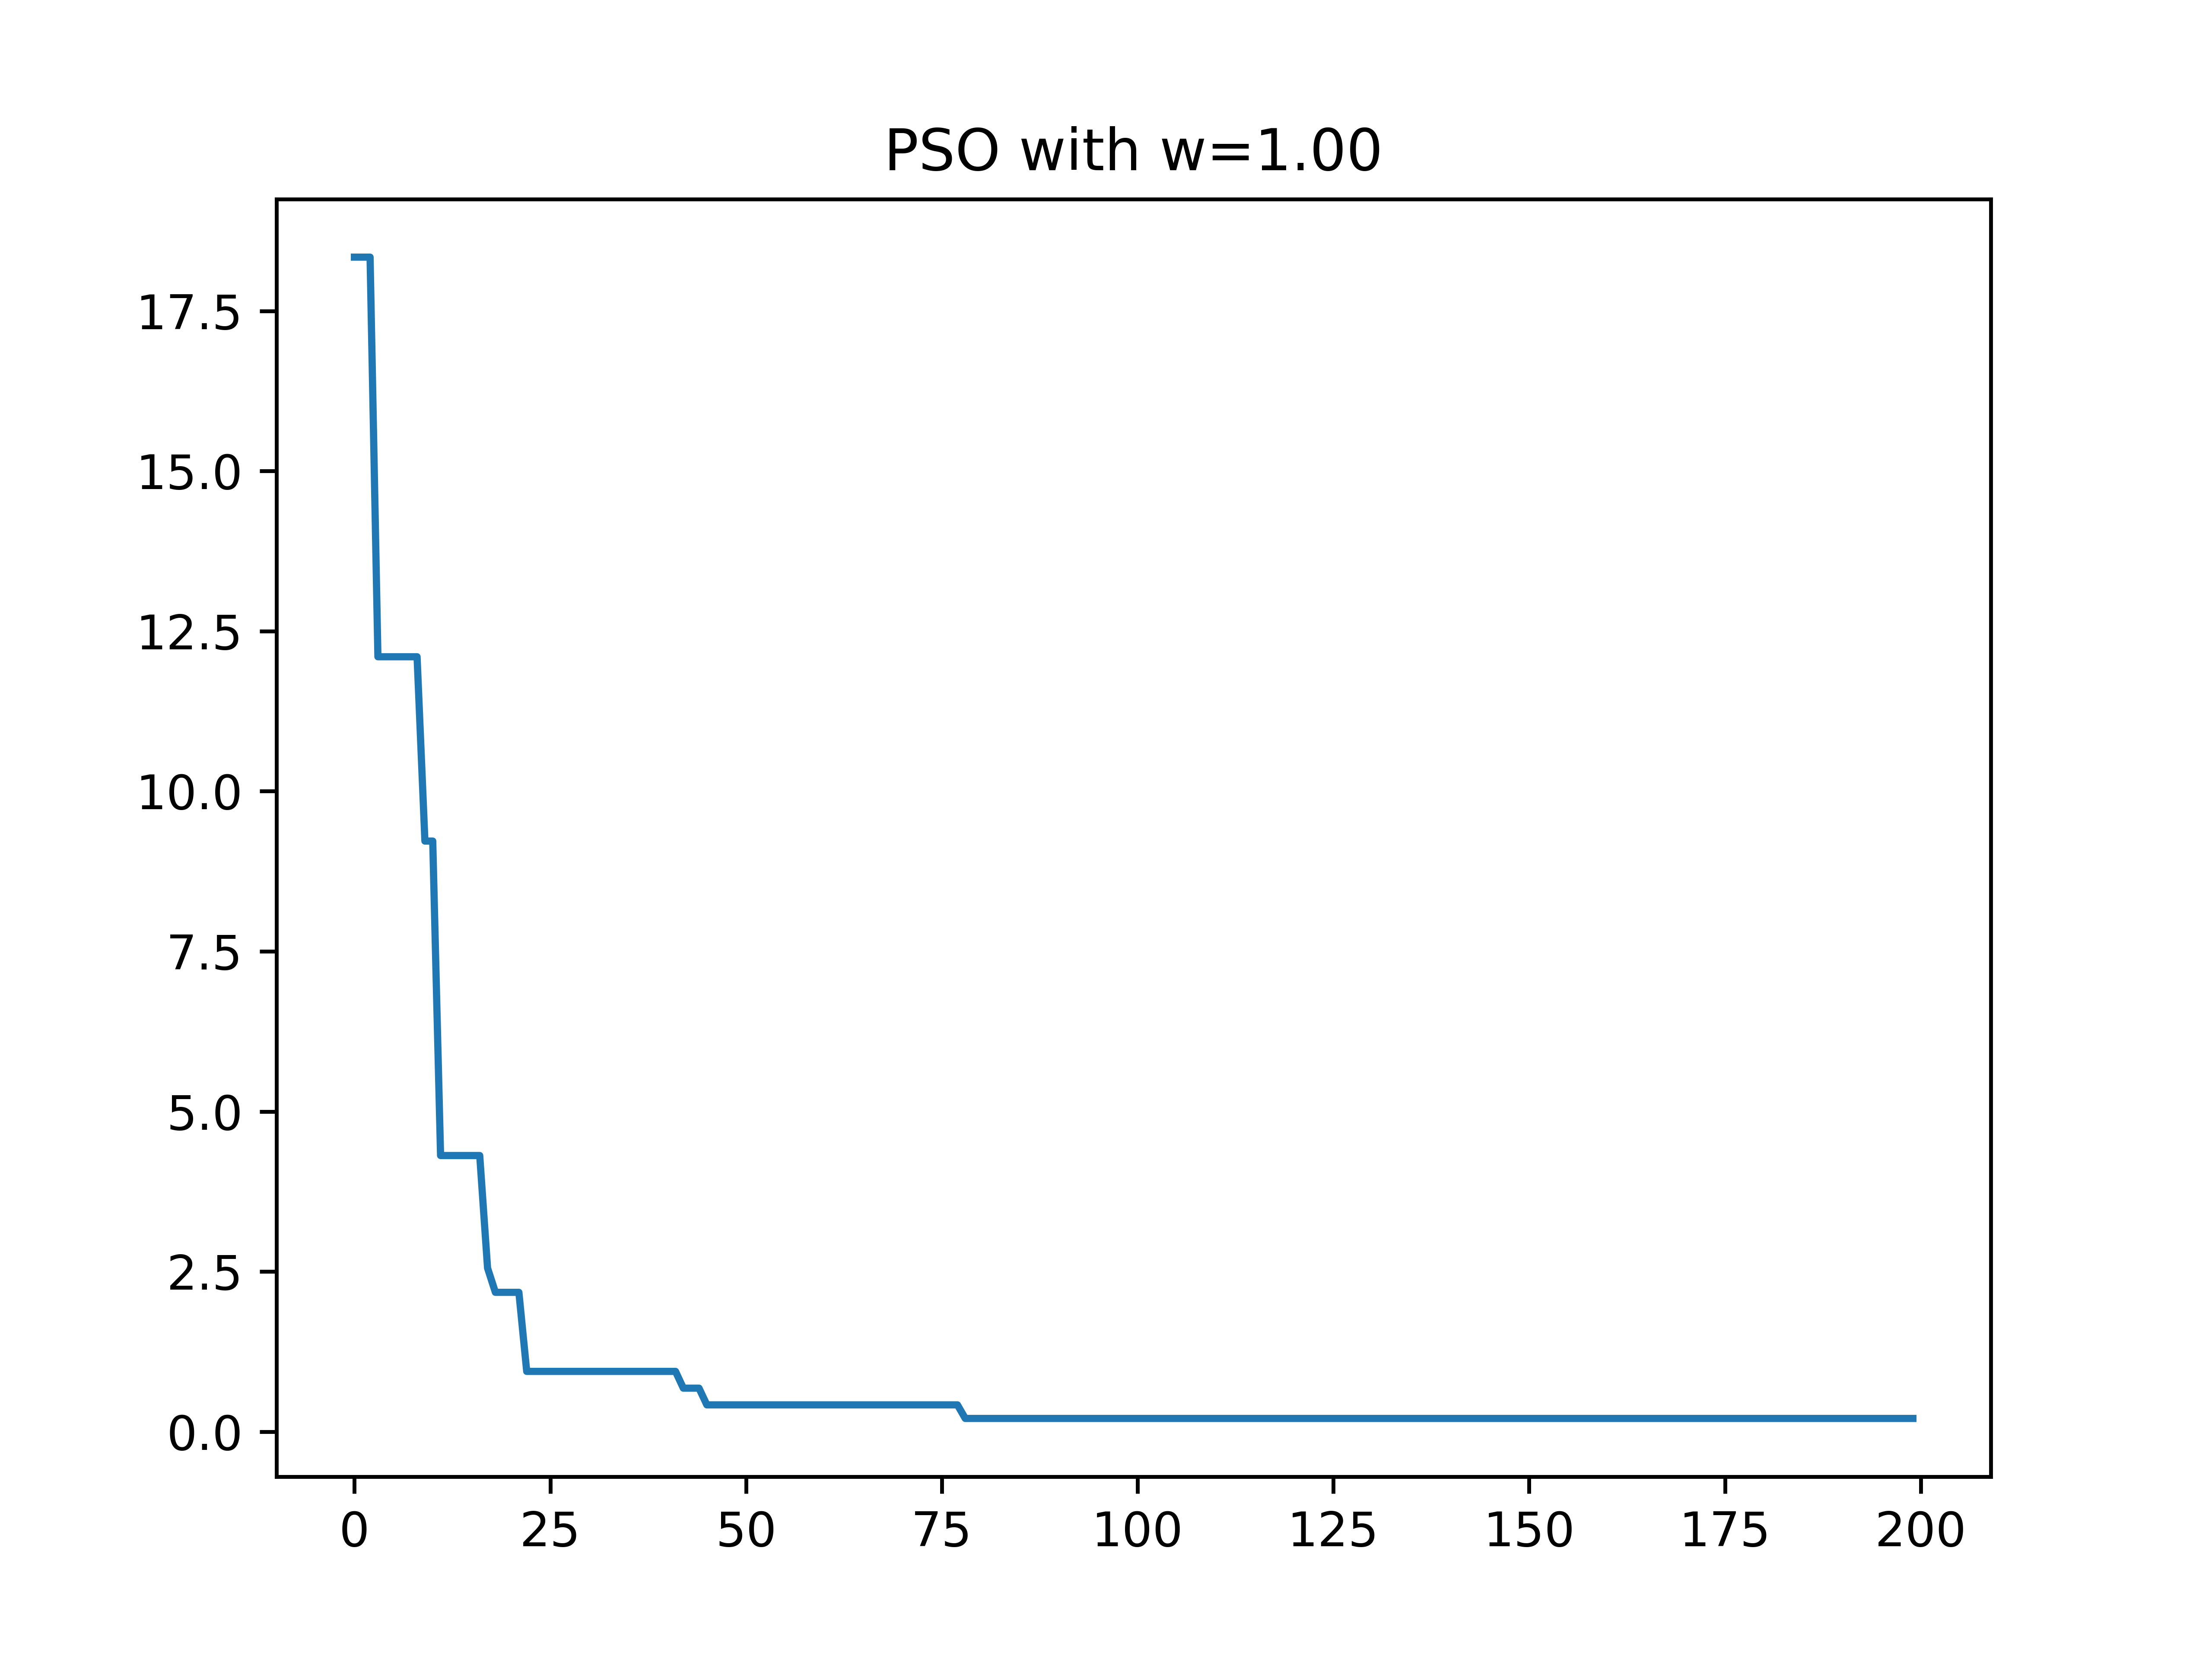
\includegraphics[width=0.6\textwidth]{image/fig1.png}
	\caption{PSO算法迭代过程目标函数值}
	\label{fig2}
\end{figure}

当然,在处理此类较为简单的优化问题时,也许采用传统的凸优化方法会更加方便高效,但PSO的优势在于处理更为复杂的、无法计算目标函数的梯度的问题,这个小的例子只是为了展示PSO的工作原理。

\subsubsection{例二}

我们进一步探究算法在实际情景中的应用。假设一生产商的产品有4道生产工序,每道工序可以选择3种不同的机器,机器所生产产品的成本$c_{ij}$、时间$t_{ij}$和质量$q_{ij}$不同,生产商的目标为在4道工序中合理选择不同种机器来达到成本、生产时间的最小化和质量的最大化。问题的优化模型为:
\begin{align*}
& \min y = w_1C + w_2T - w_3Q\\
s.t.\ & C = \sum_{i=1}^{4}\sum_{j=1}^{3} c_{ij}x_{ij}\\
& T = \sum_{i=1}^{4}\sum_{j=1}^{3} t_{ij}x_{ij}\\
& Q = \sum_{i=1}^{4}\sum_{j=1}^{3} q_{ij}x_{ij}\\
& x_{ij} = 1\ \text{if machine i is selected in task j, otherwise = 0}\\
& \sum_{j=1}^{3} x_{ij} = 1, \ \text{for } i = 1,2,3,4
\end{align*}

生产商通过AHP方法确定下三个指标的权重分别为$w_1 = 0.39$,$w_2=0.28$,$w_3=0.33$,求生产商最优的选择。

这是一个维数较高(3$\times 4=12$)的问题,且涉及到整数规划,用常规优化方法进行求解则繁琐且效率不高,现用PSO算法尝试求解。图(\ref{fig3})为目标函数值随迭代次数的变化,我们发现在本例的情况下,即使不设置整数的要求,最终的最优结果仍能收敛到整数,且在极短的迭代次数内就可以得到最优结果。如果问题的维数更高,目标函数为更复杂的非凸函数,PSO算法的优势将更加凸显。

\begin{figure}[H]
	\centering
	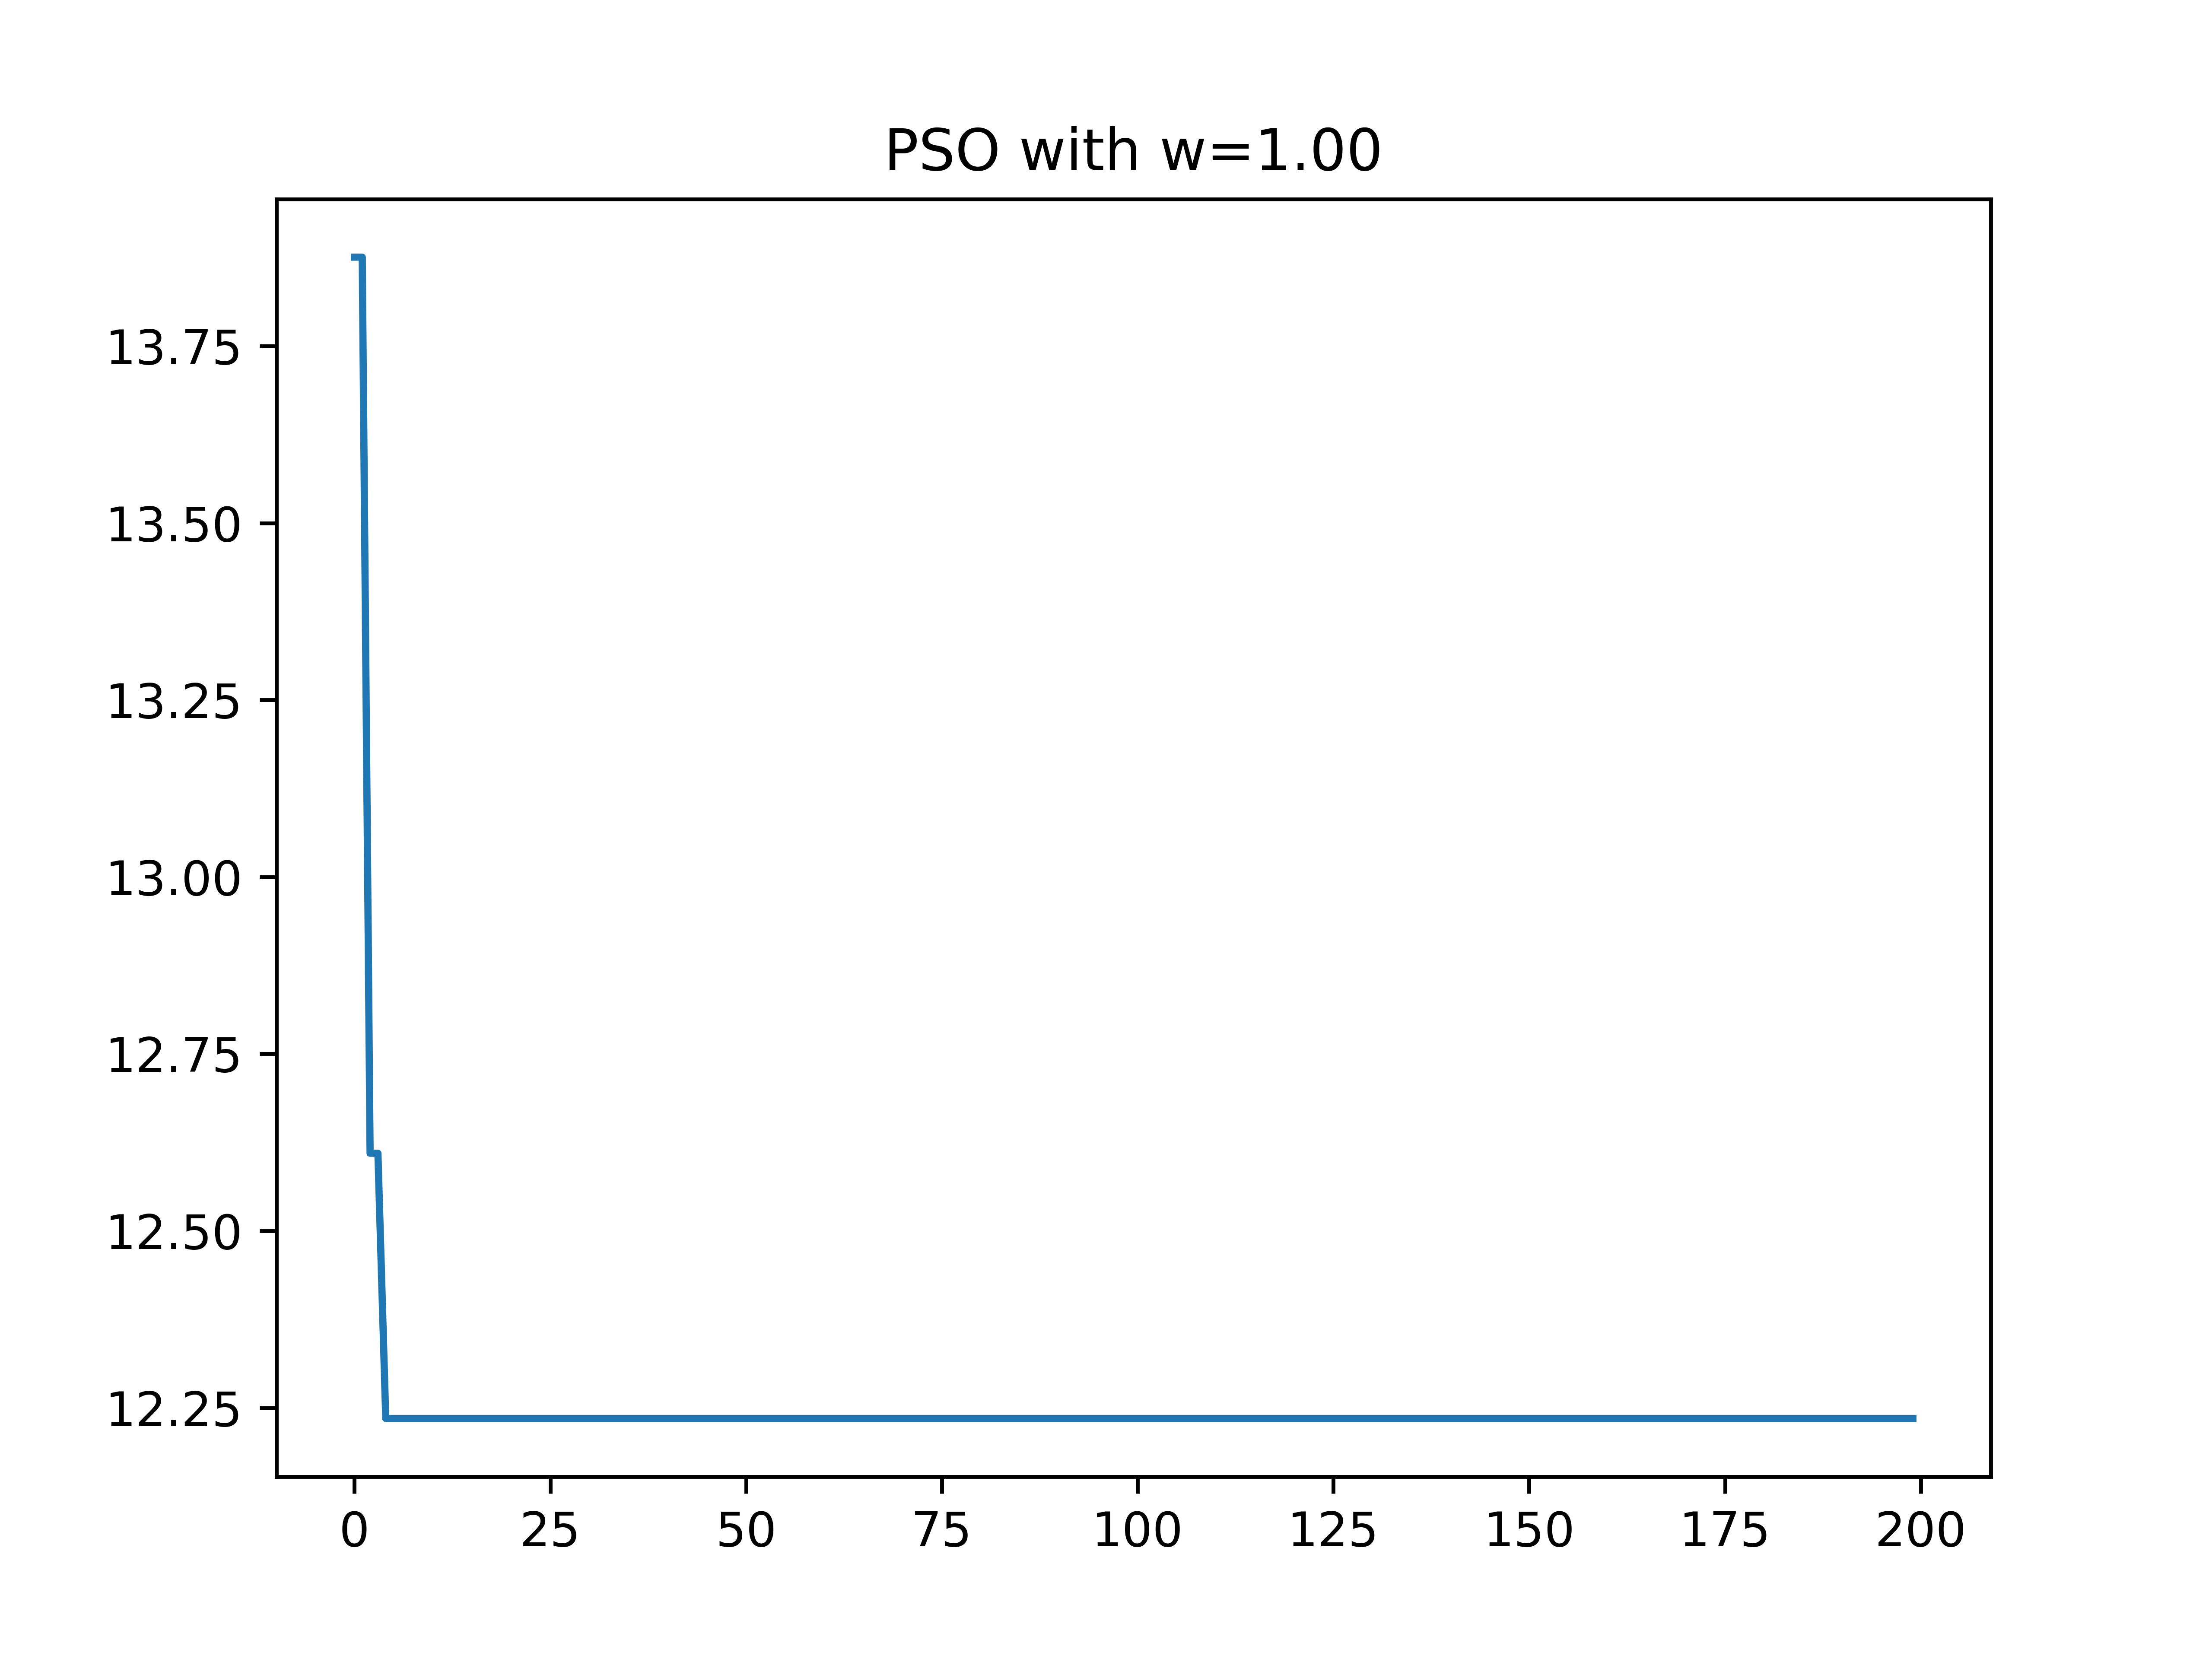
\includegraphics[width=0.6\textwidth]{image/fig2.png}
	\caption{PSO算法迭代过程目标函数值}
	\label{fig3}
\end{figure}

\section{算法发展及现状}

由于粒子群优化算法容易陷入局部最优值、搜索初期收敛速度快而搜索后期收敛速度变慢等缺点,在其提出后许多学者对其进行了完善与发展。

\subsection{添加惯性权重}

三位学者在1998年的两篇文章\citep{shi1998modified}和\citep{shi1998parameter}中引入了惯性权重(Inertia Weight)$w$,以下为加入了惯性权重的算法更新等式。
\begin{align*}
& v_{id} = w*v_{id} + c_1 * rand() * (p_{id} - x_{id}) + c_2 * Rand() * (p_{gd} - x_{id})\\
& x_{id} = x_{id} + v_{id}
\end{align*}

与最初算法中的式子相比,添加惯性权重的变化仅仅是在$v_{id}$前面乘上系数w,但选取合适的惯性权重能够更好地平衡全局与局部的开发(exploitation)和探索(exploration),于是作者将带惯性权重的PSO作为算法标准版本。

\subsection{进化优化与粒子群优化结合}

\cite{angeline1998evolutionary}将带有自然选择机制思想的进化优化(Evolutionary Optimization)引入粒子群算法中,其核心思想为:当算法更新完所有的粒子后,计算粒子的适应度值并对粒子进行适应度值排序,然后根据排序结果,用粒子群体中最好的一半粒子替换粒子群体中最差的一半粒子,但是保留原来粒子的个体最优位置信息。实验结果表明,自然选择机制的引入增强了粒子的全局寻优能力,提高了解的精度。

\subsection{添加压缩因子}

由于PSO来源于社会模型的启发,在提出时没有考虑算法的数学基础,而\cite{clerc2002particle}在1999年的研究中指出,使用压缩因子(Constriction Factor)也许能够保证算法的收敛性。其推导证明过于复杂,不在本文中讨论,简单来说,添加压缩因子即将原始算法的更新等式换为如下所示:
$$v_{id} = K*[v_{id} + c_1 * rand() * (p_{id} - x_{id}) + c_2 * Rand() * (p_{gd} - x_{id})]$$

其中$K$是$c_1$与$c_2$的函数:
$$K = \frac{2}{|2-\phi - \sqrt{\phi^2 - 4\phi}|}, \quad \text{where } \phi = c_1+c_2, \ \phi > 4$$

压缩因子的引入在控制粒子群算法收敛的同时,使得粒子有机会搜索空间中不同的区域,并获得高质量的粒子。实验结果表明,它大大提高了粒子群算法的收敛速度和收敛精度。


\subsection{自适应粒子群优化算法}

\cite{zhan2009adaptive}在2009年提出了一种自适应的粒子群优化算法(Adaptive Particle Swarm Optimization, APSO),它有着比经典粒子群优化算法更好的搜索效率,且能够以更快的收敛速度在整个搜索空间中执行全局搜索。 

APSO包含两个主要步骤:首先,通过评估种群分布和粒子适应度,执行实时进化状态估计,算法可以在运行时自动控制惯性权重、加速度系数和其他算法参数,从而提高搜索效率和收敛速度。然后,当进化状态被分类为收敛状态时,执行精英学习(Elitist Learning)策略。该策略将作用于全局最佳粒子,以跳出可能的局部最优值。 文章结果表明,APSO在收敛速度、全局最优性、解决方案精度和算法可靠性方面大大提高了PSO范式的性能,且不会引入额外的设计或实现复杂性。



\section{算法应用与展望}

\subsection{算法应用}

从前文的分析中不难看出,粒子群算法可以广泛运用于优化理论当中。而这方面的研究是当今的前沿热点,尤其是随着计算机的广泛应用,计算性能的加强,优化技术不仅成为迫切需要,而且有了有效的求解工具。在这方面,典型的理论问题包括:组合优化、约束优化、多目标优化、动态系统优化等。实际工业应用有:电力系统、滤波器设计、自动控制、数据聚类、模式识别与图像处理、化工、机械、通信、机器人、经济、生物信息、医学、任务分配、TSP等等。

在前文中,我们已经展示了粒子群算法在生产与运作管理方面的应用,可以帮助企业选择竞标公司,安排生产流水线等。下面我们再选取一些实际的例子,以展示粒子群算法在经济管理领域的应用。

\subsubsection{配送中心的选址}

在文章\citep{TN_wanfang_jourgljtkj201112026}中,作者提到,配送中心选址问题是设施选址问题的重要研究领域之一。配送中心选址决策的优劣,不仅对配送中心本身、供应商及零售商的运营成本、绩效产生重要影响,且对该地区区域经济的发展也具有突出作用。这个问题也是一个经典的运营管理的例子,也适用于使用PSO来寻求最优解。\cite{TN_springer_jour1020763400324}利用库存风险共担策略构建了适用于配送中心选址问题的非线性0-1整数规划模型。\cite{TN_informstrsc.37.1.40.12823}用拉格朗日松弛法求解该模型并获得良好计算效果。该模型假设每个零售商需求都为正态独立分布,所有零售商需求必须满足且必须由一个配送中心供货,配送中心无配送能力限制,模型不仅计算成本的最优值,即最小成本,而且求解配送中心的最优建设区位与配送中心的配送方案。\cite{TN_informstrsc.37.1.40.12823}首先利用风险共担策略将安全库存设在配送中心,进而采用EOQ 经济订货批量模型计算配送中心的最优订货量。该模型在实际中取得了良好的效果。

\subsubsection{金融风险模型}

在金融领域,学者们主要将粒子群算法应用于投资组合优化、股指收益波动率预测、金融风险预警模型构建等方面。如何有效求解基数约束投资组合优化问题,是金融学界的研究热点。例如,基于Markowitz M-V 投资组合优化问题可以以如下方式建模\citep{TN_cqvip668694543}。

假设有$N$种资产,$r_i$ 表示第$i$ 种资产的期望收益($i = 1,\cdots,N$),$\sigma_{ij}$ 表示资产$i$ 和资产$j$ 之间的协方差($i,j=1,\cdots,N$)。$x_i$ 和$\lambda$ 分别表示资产$i$ 的投资比率和投资者风险厌恶系数。基于Markowitz M-V 模型的投资组合选择问题描述为:
\begin{align*}
\min \ & \lambda[\sum_{i=1}^{N}\sum_{j=1}^{N}x_i \cdot x_j\cdot \sigma_{ij}] - (1- \lambda)[\sum_{i=1}^{N}x_i\cdot r_i]\\
s.t.\ & \sum_{i=1}^{N}x_i=1\\
& 0\leq x_i \leq 1, \ \text{for }i = 1,\cdots,N
\end{align*}

由问题的数学形式,非常容易看出,上述问题可以使用粒子群算法得到较好的解决。而事实上,使用PSO来解决Markowitz基数约束投资组合优化问题非常有效,不仅容易实现,而且优化结果符合实际要求。

\subsection{展望}

和其他算法一样,PSO是一种新兴的智能优化算法,在理论和应用方面仍然有很多值得进一步研究的方面。虽然目前对PSO稳定性和收敛性的证明已取得了一些初步成果,但自诞生以来其数学基础一直不完备,特别是收敛性一直没有得到彻底解决。因此,仍需要对PSO的收敛性等方面进行进一步的理论研究。而由于PSO本质上是一种随机搜索算法,如何提高该算法的可解释性,从而将该算法能与现有的工业技术相结合,并进行推广,还有很长的路要走。

在PSO算法研究方面,未来有如下研究方向\citep{huanglei}:

\begin{enumerate}
	\item 应用领域的拓展: 目前该算法主要应用于函数优化及神经网络的训练等领域, 而开拓新的应用领域,在应用的广度和深度上进行拓展都是很有价值的工作。
	\item 算法参数的确定: PSO中的一些参数如$c_1$、$c_2$、$w$、微粒个数以及迭代次数等往往依赖于具体问题,依据应用经验, 经多次测试来确定, 并不具有通用性。
	\item 算法的改进研究: 由于实际问题的多样性和复杂性, 尽管已出现了许多改进的算法, 但远不能满足需要,如何根据不同的问题提出相应的改进算法是研究热点。
	\item 算法的基础理论研究: PSO的数学基础相对薄弱, 缺乏深刻且具有普遍意义的理论分析, 不能对PSO的工作机理做出合理的数学解释。虽然PSO的有效性、收敛性等性能在一些实例中得到验证,但没能在理论上进行严谨推敲和严格证明。
\end{enumerate}

不可否认的是,PSO算法已经在实际中有非常广泛的应用。该算法非常简洁,结构简单,需要调节的参数少,需要的专业知识少,实现方式容易,所以在各种自然科学和工程领域中都有很多的应用,这方面的资料也非常丰富。

\section{小结}

从上述对PSO算法的探讨,我们不难发现,一个人工智能算法的成熟,除了需要在实际中得到很好的应用,而且需要有一定的可解释性、有可供选择的参数选择与指导准则,还需要有计算便捷性,理论完整性等。当然,随着人工智能领域在近年来的飞速发展,人工智能、机器学习算法的研究也朝气蓬勃,而这些领域还有很多可以完善、可以发展的部分。由于不同算法所使用工具和分析方法都有很强的相似性,因此,如果一个算法取得突破性进展,将会对整个领域产生非常重大的影响!而人工智能领域发展到现在,上述问题难度较大,也是迫切需要解决的问题。实际中这类问题往往增加很强的假设条件,或者神经网络深度过大,这还有很大的改进空间。

近年来,交叉学科的发展逐渐成为主流。对于信管的同学来说,信息管理,计算机科学,运筹学,数学,统计学等学科都需要深入了解,这能丰富我们的知识,做出有价值、有意义的成果。多领域的交叉发展是大势所趋,而学习粒子群算法等人工智能有关的知识,可以运用在生产与生活当中。特别地,如涉及到生产运作,决策理论,运筹学,优化,机器学习,人工智能,计算机技术等领域时,也可以使用人工智能的算法,探索问题的解,启发新的思路。




\newpage
\nocite{*}
\bibliography{paper1}

\newpage
\appendix
\appendixpage
\addappheadtotoc

例一的Python代码实现:

\begin{lstlisting}[language=Python]
from sko.PSO import PSO
import matplotlib.pyplot as plt

def demo_func(x):
	x1, x2 = x
	return (x1 ** 2 + x2 ** 2)/100.0

def pso_opt(w=1):
	pso = PSO(func=demo_func, dim=2, pop=50, max_iter=200, lb=[-300, -300], ub=[300, 300], w=w, c1=0.5, c2=0.5)
	pso.run()
	print('best_x is ', pso.gbest_x, 'best_y is', pso.gbest_y)
	figure, ax = plt.subplots(1, 1)
	ax.plot(pso.gbest_y_hist)
	ax.set_title("PSO with w=%.2f"%w)
	plt.show()


if __name__ == "__main__":
	pso_opt()

\end{lstlisting}

例二的Python代码实现:

\begin{lstlisting}[language=Python]
from sko.PSO import PSO
import numpy as np
import pandas as pd
import matplotlib.pyplot as plt

m_cost = [[2, 1, 3],
			[3, 3, 5],
			[6, 3, 3],
			[9, 8, 6]]
m_time = [[2, 1, 1],
			[6, 3, 2],
			[4, 3, 5],
			[5, 7, 6]]
m_quality = [[9, 8, 9],
			[5, 7, 6],
			[8, 7, 5],
			[7, 7, 8]]
m_cost = np.mat(m_cost)
m_time = np.mat(m_time)
m_quality = 10 - np.mat(m_quality)
w = [0.39, 0.28, 0.33]

def obj_func(x):
	x_mat = np.mat(x)
	x_mat = np.reshape(x_mat, (4, 3))
	x_mat = pd.DataFrame(x_mat)
	temp = x_mat.apply(lambda y: y/sum(y), axis=1)
	x_mat = np.mat(temp)
	func_value = w[0]*np.multiply(x_mat, m_cost) + w[1]*np.multiply(x_mat, m_time) + w[2]*np.multiply(x_mat, m_quality)
	return func_value.sum(axis=0).sum(axis=1)[0, 0]

def run_pso(w=0.8, c1=0.5, c2=0.5):
	pso = PSO(func=obj_func, dim=12, pop=50, max_iter=200, lb=[0]*12, ub=[1]*12, w=w, c1=c1, c2=c2)
	pso.run()
	print('best_x is ', pso.gbest_x, 'best_y is', pso.gbest_y)
	figure, ax = plt.subplots(1, 1)
	ax.plot(pso.gbest_y_hist)
	ax.set_title("PSO with w=%.2f"%w)
	plt.show()


if __name__ == "__main__":
	run_pso(w=1, c1=2, c2=2)
\end{lstlisting}


\end{document}
